\chapter{隐私保护}
\label{chap:trust-privacy}

一封私人邮件被用于训练垃圾邮件分类器，本意是改进服务，却可能在多个环节造成意料之外的信息暴露。开发者为审计公平性收集的群体属性同样敏感；即使从不公开原始邮件，训练后发布的模型参数和它给出的回答仍可能泄露训练内容；用户日后要求撤回邮件时，删掉文件也不会自动抹除模型已经学到的影响。隐私问题因此贯穿数据进入系统、参与训练、对外发布和被删除的整个生命周期。

用第~\ref{chap:trust-foundations}章的三层框架看，隐私首先是一条需要写成规范要求的系统属性：哪些人的哪些信息可以由谁访问、使用或获知。第二层要判断证据能否支持这条要求，靠的是泄露审计、形式化分析和实现核查。第三层关注运行过程：授权和数据流边界要持续执行，多次发布的隐私消耗要累计，用户撤回数据时要有处置流程。

本章沿这条线回答四个问题。要保护什么、可能从哪里泄露、保护强度怎样度量，这是讨论一切措施的前提（第~\ref{sec:privacy-concepts}节）；有了承诺，就要知道怎样检查它是否兑现（第~\ref{sec:privacy-verification}节）；检查暴露出缺口后，再看采集、训练、发布和预测各环节有哪些保护手段（第~\ref{sec:privacy-use}节）；最后处理数据进入模型之后的撤回（第~\ref{sec:privacy-unlearning}节）。贯穿全章的还有公平审计与隐私的张力：把群体切细有助于发现集中的伤害，却也可能暴露人数很少的群体成员。

\section{隐私保护的基本概念}
\label{sec:privacy-concepts}

\subsection{保护对象与保护范围}
\label{sec:privacy-subjects}

用户把邮件交给分类器时，系统获得的信息可能不止该用户自己的，还包括发件人、收件人和邮件里提到的其他联系人。提交者有权使用接口，不代表这些第三方的信息可以任意公开。机器学习中的\term{隐私保护}（privacy protection）研究的就是：在完成任务的同时，如何限制个人信息受到不适当的访问、使用、推断和披露。保护对象因此要覆盖三类人：训练样本的提供者、当前请求的使用者，以及内容中涉及但并未表示同意的第三方。

讨论保护强度前，要先分开两个常被混为一谈的问题。第一个问题是“要藏什么”，即希望保密的事实，例如“这封邮件是否参加了训练”、邮件中的私人编号，或本次请求携带的地址。第二个问题是“保护谁的数据”，即保护单位，例如一条记录，或同一用户的全部记录。前者决定要阻止观察者获知什么，后者决定要限制谁的数据对发布结果产生影响。两者回答不同的问题：一封邮件得到某种强度的保护，不能推出同一用户的一万封邮件合在一起仍有同等强度的保证，因为一万封邮件对结果的合力可能远大于一封。

这与第~\ref{chap:trust-fairness}章的视角不同：那里按群体比较预测误差，这里按记录或用户规定保护单位。按群体报告效用损失，不等于该群体作为一个整体也享有相同隐私参数的保证。同一人的多条记录怎样归集、共同记录里的其他人是否纳入保护，也都要写明；仅凭账户归属关系不足以确定全部保护对象。

后文固定一个受控例子：邮件$z$含一个私人项目编号，训练集$D$包含这封邮件，分类器训练后开放查询。围绕它可以问三个问题：查询者能否判断$z$是否参加了训练（成员身份），能否从输出复现编号（内容），训练服务器能否借共享的梯度更新恢复内容（中间状态）。如果用户撤回的是全部邮件而非一封，处置范围就应包括所有可定位的相关记录和衍生状态。

一条可以核查的隐私承诺应逐项列明：涉及哪些人、哪些私人事实、用于什么目的、允许的接收者是谁、通过哪些系统接口可见。例如，模型可以为收件人整理邮件，但这并不授予它把地址传给无关工具的权限。判断隐私是否得到保护时要逐项核对这些范围；“这条样本曾经公开过”只是背景信息，不能单独决定结论。

\subsection{机器学习中的泄露途径}
\label{sec:privacy-leakage-channels}

有了保护对象，下一步是找出信息可能从哪里流出。沿这封邮件的数据流可以找到多个暴露点：原文可能在采集、传输或存储时被无权者读取；训练中的梯度、检查点和调试日志可能透露具体样本；发布的参数和查询回答可能保留训练信息；预测时另行提供的私人上下文，还可能进入检索结果、工具调用、回复和服务日志。每个位置都要说明观察者能看到什么，用户看到的最终回答只是其中一个接口。

泄露审计按“观察者想获知什么”分类，而不按处理阶段划分。\term{成员推断}（membership inference）判断某条记录是否参加了训练；属性推断（attribute inference）预测未公开的字段；数据重构（data reconstruction）尝试恢复完整输入；训练数据提取（training data extraction）通过反复查询诱导模型复现训练片段。这几类攻击可能共用同一渠道：训练更新既能用于重构输入，发布的模型既能用于判别成员，也能用于提取内容。

泄露并不要求模型把原文逐字存下来。只要训练成员和非成员在模型分数上的分布略有差别，这种差别就可能成为判断成员身份的线索；参数也可能保留训练中偶然出现的罕见片段。“预测正确”与“记忆”之间也没有必然联系：模型可以只凭一般语言规律正确分类，并不记得某封邮件；也可能记住了罕见编号，却在当前分类任务上预测错误。审计因此要分清三种信息：观察者原有的知识、公开的普遍规律，以及使用了私人数据后额外获得的信息。

把记录留在本地，只能阻止原文沿某一条路径直接传输。如果上传的梯度足以重构输入，或发布的模型保留了私人片段，信息照样会从其他路径流出。同理，把原文表示成向量、梯度或统计量，也不能仅凭“形式变了”就证明保密，这些表示可能比想象中更容易反推。检查要分别覆盖原始访问权限、中间计算状态和最终输出三处。

即使完全没有训练记忆，当前这一次请求也可能泄露信息：模型把用户刚提交的私人编号发给无权接收的工具，这一刻就已经越过信息边界，无需事先用它训练。公开网页上的内容能否再次披露，同样要结合使用情境判断，不能因为“来自公开网页”就任意转发。用途和接收范围由第~\ref{sec:trust-context}节的情境规定，不能只凭内容来源推断。

\subsection{保护承诺与强度}
\label{sec:privacy-guarantees}

前两小节列出了要藏的事实和可能的出口。访问规则规定谁能读取和操作数据，协作计算规则规定参与方能看到哪些中间状态；但这两类规则都管不到一件事：一个被授权获得统计量或模型的人，能从中反推出多少私人信息。下面先用一个例子说明这个缺口，再给出填补它的形式化定义。

\paragraph{精确统计量的缺口}

设查询者已经知道除$z$以外的所有邮件，服务公布“含某关键词的邮件数”的精确计数。若$z$含该词，加入它使计数从$c$变成$c+1$。查询者对比自己掌握的$c$和公布值，就能确定$z$是否存在。查询经过授权、答案名义上只是一个统计量，都不能削弱这种确定性的区分能力。问题出在发布值是数据的确定函数：只要一条记录改变了它，观察者就能看出差别。

\paragraph{差分隐私的定义}

要让“某条记录是否参与”难以从发布值判断，可以让发布结果带有随机性，并限制单个受保护对象对输出\emph{分布}的影响：比较“数据集包含该对象”和“不包含该对象”两种情形时，同一个输出事件出现的概率不能相差太大。\term{差分隐私}（differential privacy, DP）把这个要求写成一条对所有情形统一成立的不等式。

先按保护单位约定什么叫两个“相邻”数据集，记作$D\sim D'$，通常指两者相差一条记录或一个用户的全部记录。随机发布算法$M$满足$(\epsilon,\delta)$-差分隐私，当且仅当对每一对相邻数据集和每个可测输出事件$E$都有
\begin{equation}
 \mathbb P\bigl(M(D)\in E\bigr)
 \leq e^\epsilon\mathbb P\bigl(M(D')\in E\bigr)+\delta\, .
 \label{eq:privacy-dp-definition}
\end{equation}
这里$\epsilon\geq0$、$\delta\in[0,1)$，概率只来自发布算法自身的随机性，数据集是固定的。$e^\epsilon$是允许的概率倍数：$\epsilon=0.1$时$e^{0.1}\approx1.105$，意味着任何输出事件在两种数据下的概率至多相差约10.5\%；$\epsilon=0$意味着输出分布完全不受这条记录影响。$\delta$是在倍数约束之外额外容许的一小块概率。邻接关系是对称的，交换$D,D'$后同样要满足该式；它是对每一对数据和每个事件都成立的要求，而不是只针对某一次攻击或平均情形。$\delta=0$时称为纯差分隐私，$\delta>0$时称为近似差分隐私。

用计数例子检验这个定义。取包含$z$的$D$、不含$z$的$D'$，事件$E$为“输出正好是$c+1$”。精确机制在$D$下该事件概率为1，在$D'$下概率为0，不等式要求$1\leq e^\epsilon\cdot0+\delta=\delta$，任何$\delta<1$都不成立。这就严格说明了精确计数不可能满足差分隐私，必须让发布值随机化，使两种数据下的输出分布充分重叠。定义只规定概率变化的限度，不指定具体的加噪算法；用什么机制达到它是机制设计问题，机制与实现是否相符则由验证检查。

相邻关系同时决定了保护单位。记录级可以定义为增加、删除或替换一条记录；用户级则是改变同一用户的全部记录。在同一约定下，减小$\epsilon$和$\delta$会加强限制。但$\delta$不能读成“每个用户以该概率被完全公开”：它是对整个概率不等式的容忍量，不是按人抽签。

差分隐私的保护范围也有边界。它限制的是“因为使用了受保护数据而额外泄露的信息”，人口层面的公开规律照样可以用于推断：即使完全没读过某人的数据，观察者也能依据其所属人群的共同统计特征对他作出判断，这部分推断差分隐私不消除。差分隐私也不保证预测正确。理解一条差分隐私结论，必须连同保护定义、实现机制和组合分析一起看\scite{dwork2014privacy}。

\paragraph{从假设检验理解参数}

$\epsilon$和$\delta$究竟限制了观察者什么？可以把观察者看成在做一次成员假设检验。设$D$比$D'$多一条待检记录，观察者在输出落入事件$E$时判为“参加了训练”。这个检验的真阳性率为$t=\mathbb P(M(D)\in E)$，假阳性率为$f=\mathbb P(M(D')\in E)$。代入式~\eqref{eq:privacy-dp-definition}，纯差分隐私要求$t\leq e^\epsilon f$，近似差分隐私要求$t\leq e^\epsilon f+\delta$。由于$E$可以是任意事件，这条约束对观察者能设计的所有检验都成立，而不只限制某个已知攻击的平均准确率。例如$\epsilon=1$、$\delta=0$时，假阳性率为1\%的检验，真阳性率至多约2.7\%：观察者无法同时做到“很少冤枉非成员”和“经常识别出成员”。

\paragraph{多条记录同时变化}

一次改变多条记录时，不能直接套用单条记录的隐私参数。设两个数据集相差$k$条记录，可以在它们之间插入$k-1$个中间数据集，使相邻两个只差一条。先看$k=2$：设中间数据集为$D_1$，对$(D,D_1)$和$(D_1,D')$各用一次定义，得到
\[
 \mathbb P(M(D)\in E)\leq e^\epsilon\bigl(e^\epsilon\mathbb P(M(D')\in E)+\delta\bigr)+\delta
 =e^{2\epsilon}\mathbb P(M(D')\in E)+\delta(1+e^{\epsilon}).
\]
每多走一步，前面累积的项都会再乘一次$e^\epsilon$，再加一个新的$\delta$。照此递推$k$步得到
\begin{equation}
 \mathbb P(M(D)\in E)
 \leq e^{k\epsilon}\mathbb P(M(D')\in E)
   +\delta\sum_{j=0}^{k-1}e^{j\epsilon}.
 \label{eq:privacy-group-bound}
\end{equation}
这个界显示参数随$k$迅速退化：倍数从$e^\epsilon$变成$e^{k\epsilon}$。例如一名用户最多提交一百封邮件，“该用户是否参与”最多对应一百步记录级相邻变化，记录级$\epsilon=0.1$对用户而言只剩$e^{10}$倍的概率约束，几乎没有保护。要按用户保护，就要限制每名用户所有贡献的总量或按用户裁剪，这会改变需要分析的敏感度。

\paragraph{观察者与信任边界}

上面的定义还隐含一个前提：谁在什么时候能看到明文。中心化差分隐私假设存在一个可信管理者，他先看到全部明文，再发布受保护结果。如果用户不信任服务器，这个前提就不成立。替代做法是在数据离开用户设备之前就随机化，称为\term{本地差分隐私}（local differential privacy）：每个用户先给自己的数据加入随机性，服务器只收到随机化后的消息。形式上，本地随机化器$R$对任意两个输入$x,x'$和任意消息事件$E$满足
\[
 \mathbb P(R(x)\in E)
 \leq e^\epsilon\mathbb P(R(x')\in E)+\delta.
\]
它与式~\eqref{eq:privacy-dp-definition}的形式相同，只是比较对象从“相邻数据集”换成了“单个用户的任意两个取值”。

这个承诺是关于消息分布的统一界，不等于每条消息都绝不透露输入。允许$\delta>0$时，一个机制可以以概率$\delta$直接发送输入、其余时候发送固定符号：对“消息等于$x$”这一事件，两种输入下的概率分别为$\delta$和0，恰好满足$(0,\delta)$-本地差分隐私，却会在前一种消息出现时完全透露输入。因此报告时必须同时给出$\epsilon$和$\delta$。本地方案的代价是每个用户独立加噪，汇总估计要承担比中心化方案大得多的噪声。两种安排的区别在于明文能被谁接触；具体的本地发送机制见第~\ref{sec:privacy-collection}节。

\section{隐私保护的验证}
\label{sec:privacy-verification}

有了承诺和度量，接着要问：怎样知道这封邮件实际有没有泄露？有两条互补的取证路径。结果检验从可见输出（回复、分数、参数、共享更新）出发，让观察者在指定权限下尝试恢复私人事实；过程核查沿处理过程检查数据流、授权、随机机制和发布步骤是否符合承诺。前者能发现已经可被利用的泄露，后者能发现尚未被攻击利用但确实存在的缺口。两者都不能代替形式化保证所需的证明，后者必须论证对全部允许输入成立。

\subsection{基于可见结果的泄露检验}
\label{sec:privacy-leakage-audit}

经验审计让属性推断、成员推断、内容提取或输入重构等攻击尝试利用指定接口。要让结果可以解释，攻击者的背景知识、查询预算、先验分布和评价数据必须事先固定，结果才能与“随机猜测”和“仅凭公开规律”两条基线比较。候选来源尤其要控制：成员样本和非成员样本若来自不同时间或不同数据源，攻击识别出的可能只是来源差异，而不是训练参与。

秘密和接口共同决定审计问题：未公开属性要比较看了输出后推断能力提高了多少；训练参与要判别成员；发布模型中的私人片段要做提取测试；共享更新要做输入重构测试。每项结果都应同时报告恢复了什么、需要什么权限、误报多少、查询成本多少，攻击成功率才有意义。下面按从直接到间接的顺序逐项讨论。

\paragraph{原文与字段的直接暴露}

先查最直接、不需要任何推断的泄露，例如公开日志写出了地址，工具请求带上了不必要的私人编号。可以在隔离测试中插入带合成私人标记的输入，保存输入、回复、工具参数和所有可访问日志，追踪标记最终到达哪些接收者。测试要覆盖不同账户权限和处理分支，并预先规定允许的数据流。标记越界即可确认该路径泄露；没发现标记只支持“已查路径未泄露”，还要用后面的攻击检验没有直接给出原文时能否间接恢复。

\paragraph{未公开属性的推断}

对未公开字段，关键比较是：看到模型输出之后，是否比仅凭原有知识更容易推断。例如观察者已知邮件主题和发送时间，想判断私人项目类别。基线攻击器只用这些已知量，另一个攻击器在此基础上加入模型分数或表示，两者在同源的独立样本上评价。属性目标、先验、可见接口和查询预算必须一致，否则准确率上升可能只是因为模型偏向多数类别。

这种比较支持的是“接口新增了推断能力”的证据，它与差分隐私限制的“参与影响”是两回事。人口规律可能让一个从未参加训练的人也被推断出属性：若观察者原本已知这些规律，单凭它们得到的判断应计入基线；若接口新提供了观察者原来不知道的规律，即使对非成员也会增加推断能力，而差分隐私并不禁止发布总体规律。攻击没超过基线，只说明在当前知识和预算下没发现额外信息。除总体准确率外，还应报告各属性取值和各群体的错误率、攻击器赋给真实属性值的概率及其校准误差，不能凭一个平均数宣布属性已泄露或已受保护。

\paragraph{训练成员身份的判别}

成员推断要利用的线索是：模型在训练样本上通常拟合得更好，损失较低。但样本本身难度不同，有的非成员也很容易预测，所以用一个统一的置信度阈值未必能把成员区分开。Shokri 等提出影子模型方法来学习更细的差异模式：攻击者用成员身份已知的辅助数据训练若干“影子模型”，模拟目标模型的训练过程；由于知道影子模型的训练集，就能收集成员和非成员在输出上的差异，再训练一个判别器。这样攻击者即使只能查询目标模型，也可能获得成员证据\scite{shokri2017membership}。

受控且获授权的审计可分四步执行：
\begin{enumerate}
 \item 在同一来源准备候选，记录哪些候选记录实际被纳入目标模型的训练样本；攻击器训练样本与审计评价样本分别保存。
 \item 用辅助数据训练影子模型，取得已知成员和非成员的损失、预测概率等特征，再以成员标记训练攻击器。
 \item 从目标接口取得同类特征，在验证样本上选择阈值，到独立审计样本分别计算成员命中率与非成员误报率。
 \item 固定查询预算，与不读取目标输出的基准比较，并报告低假阳性区域、实际成员先验及敏感子群结果。
\end{enumerate}
这样得到的是可以检验的身份判定；但单条记录的高置信度仍不能单独证明训练记忆，还要结合下面的逐记录比较和成员先验。

图~\ref{fig:trust-membership-inference}沿候选记录、查询特征、成员判定展示了这套受控流程；目标成员真值只用于最终核验，不进入攻击器输入。

\begin{figure*}[!htb]
  \centering
  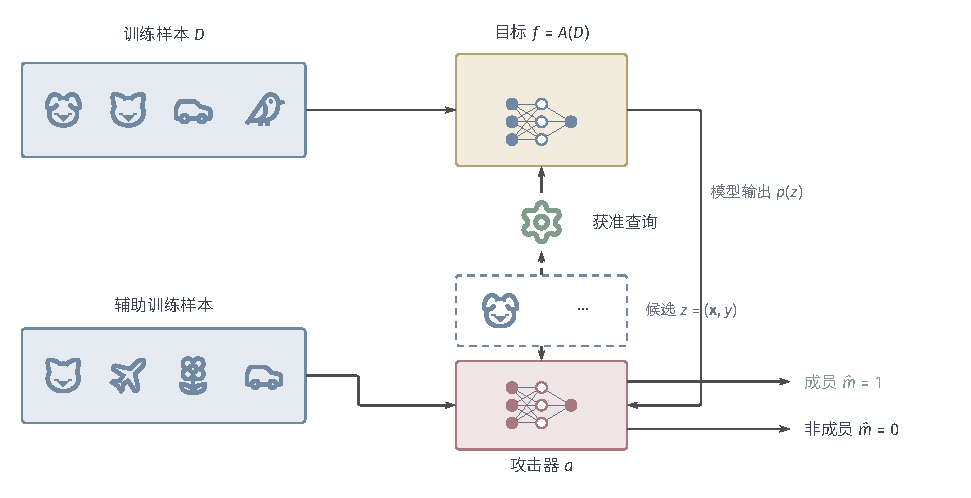
\includegraphics[width=164.600mm]{figures/03-foundations/03-trustworthiness/tikz/membership-inference/figure.pdf}
  \caption{成员推断的受控审计流程。候选成员与非成员按同一分布抽取，目标模型仅用$D$训练；记录$z=(\bm x,y)$经获准查询取得输出。图标个数表示分组，不表示成员先验；已知真实$y$时可以计算损失。攻击器用辅助成员数据训练，在验证样本上定阈值，并在独立审计样本上统计成员命中率和非成员误报率。目标成员真值用于核验，不能作为攻击器输入。该流程不承诺攻击成功，还须报告权限、查询预算与成员先验。}
  \label{fig:trust-membership-inference}
\end{figure*}

影子模型学到的成员差异能否迁移到目标模型，取决于影子训练是否真实代表目标训练；数据增强、早停或分布差异都可能让学到的规律失效。总体攻击准确率低也未必无害，攻击可能在少数敏感记录上成功率很高。因此平均值要和逐记录、逐类别以及低假阳性区域的结果一起报告。

\paragraph{逐记录的似然比检验}

影子模型对所有记录共用一套判别规则，仍会混淆“本来就容易预测”和“因参加训练才得高分”。Carlini 等的\term{似然比攻击}（Likelihood Ratio Attack, LiRA）把判断做到逐记录粒度：对每条记录分别估计“包含它训练”和“不包含它训练”时它的分数分布，再看目标模型实际给出的分数更支持哪种情形，并强调在很低假阳性率下报告真阳性率\scite{carlini2022lira}。

令记录$z$的观测分数为$s$，包含与不包含它训练时分数的条件密度分别为$p_{\mathrm{in}}(s\mid z)$和$p_{\mathrm{out}}(s\mid z)$。比较两种解释的相对可能性，就是计算似然比
\begin{equation}
 \Lambda_z(s)=
 \frac{p_{\mathrm{in}}(s\mid z)}
      {p_{\mathrm{out}}(s\mid z)}.
 \label{eq:privacy-membership-likelihood}
\end{equation}
比值大于1，说明观测分数在“参加训练”的假设下更常见。分母为零、分子为正时取$+\infty$；两个密度都为零的分数在两种假设下都不会出现，该处取值不影响检验。对两个完全指定的简单假设，按似然比大小作判定、并在判定边界随机化的检验，在给定假阳性率下具有最大功效，这就是奈曼--皮尔逊引理的结论（相关检验理论可参考\BookChapterRef{chap:statistical-inference}{卷2《数学准备：概率、因果与决策》的“统计推断”章}）。实践中两个密度只能用有限次辅助训练估计，经验 LiRA 不能直接继承这种最优性。

逐记录比较的价值可以用一个对照说明。同样是0.95的预测概率，一封普通邮件在两种假设下都容易得到这个分数，似然比接近1，不构成成员证据；一封罕见邮件只有参加训练时才常得到该分数，似然比才明显大于1。影子模型提供了学习成员规律的一般流程，LiRA 在此基础上明确了逐记录的双假设比较。

\begin{example}[成员先验改变结果的含义]
\label{ex:privacy-membership-prior}
示例~\ref{ex:privacy-membership-prior}说明先验为什么关键。候选中真实成员仅占1\%，检验真阳性率0.8、假阳性率0.1。一万条候选中预计检出$10000\times0.01\times0.8=80$个真实成员，却同时误报$10000\times0.99\times0.1=990$个非成员；全部告警中真正的成员只占约$80/(80+990)\approx7.5\%$。同一个检验在成员、非成员各占一半的平衡数据上，告警中成员比例为$0.8/(0.8+0.1)\approx89\%$。两者差别完全来自先验，因此必须报告实际先验，不能只搬用平衡测试集上的指标。
\end{example}

\paragraph{发布模型中的训练数据提取}

知道一封邮件参加了训练，只得到一个二元事实；恢复其内容则可能泄露整段私人信息，威胁大得多。Carlini 等在 GPT-2 上研究如何通过查询复现训练序列，区分“模型给某段文本的概率高”和“真的能把文本提取出来”，发现发布模型确实可能暴露训练片段，而平均泛化误差无法反映这种风险\scite{carlini2021extraction}。

模型生成一句常见话，不等于恢复了特定训练内容。受控实验可以加入来源唯一的合成标记，再检验能否复现；真实数据实验则需核验来源、去重并与对照语料比较。合成标记便于比较机制，但可能不同于自然记忆；真实内容更贴近应用，却可能混入公开重合或猜测。报告要保留这两类证据在强度上的差别。

邮件例子可以这样设计。先生成一个不含任何真实个人信息、来源唯一的项目编号，只写入指定训练邮件，并保留不含该编号的对照语料。训练后固定提示组、解码规则和一次完整试验的查询预算$k$，保存全部输出，统计准确复现次数。随机解码时用独立种子重复整次试验，以“至少提取一次的试验比例”估计该预算下的成功率；确定性解码直接报告实际结果，因为重复得到相同输出不增加证据。还要与未训练该邮件的模型比较，自适应修改提示所花的查询也计入预算。结论只说明“在指定策略下可提取”，不能穷尽模型内部是否还以其他形式保有信息。第~\ref{sec:privacy-unlearning-validation}节的遗忘审计可以复用同一套提示和预算。

\paragraph{共享更新中的输入重构}

前两项审计针对发布后的模型；在协作训练中，参与方上传的更新在训练中途就被他人看到。Zhu 等的梯度深度泄露（deep leakage from gradients, DLG）在已知模型和梯度时，搜索候选输入和标签，使它们产生的梯度与观测梯度相近，从而恢复私人样本\scite{zhu2019dlg}。这说明梯度不能当作“天然匿名的摘要”，恢复程度仍取决于模型、批次和共享方式。

线性模型给出一个可以手算的例子，说明梯度为什么会携带输入。预测为$\bm w^\top\bm x+b$，单条记录的平方损失为$\ell=\tfrac12(\bm w^\top\bm x+b-y)^2$，记残差$r=\bm w^\top\bm x+b-y$。由链式法则，权重梯度为$\nabla_{\bm w}\ell=r\bm x$，偏置梯度为$\partial\ell/\partial b=r$。权重梯度是输入$\bm x$乘上一个标量，只看到它，观察者已经知道$\bm x$的方向；若两种梯度以同一未聚合尺度公开且$r\ne0$，逐坐标相除就能还原$\bm x=\nabla_{\bm w}\ell/(\partial\ell/\partial b)$。多条样本求和、裁剪、加噪或不含偏置都会改变恢复条件。这个例子不说明任意模型都能被精确恢复，而说明“没有传原文”仍可能传出内容；保护要针对实际可见的更新，不能只检查请求里有没有原始字段。

重构审计应固定已知模型、更新轮次、批次大小和辅助信息，并在受控数据中保留真实输入作参照。恢复结果既要与真值比，也要与“仅凭公开先验猜测”比。图像外观相似、文本主题接近、私人字段精确一致，是三种不同强度的证据：恢复出常见结构不足以确认是某条特定记录，少量私人字段被精确恢复也不能因整体误差大而忽略。

\subsection{基于数据流与实现的过程核查}
\label{sec:privacy-implementation-verification}

结果检验只能覆盖试过的攻击。过程核查换一个方向，把隐私承诺逐项对应到数据流和执行条件。直接访问部分检查采集字段、身份权限、存储副本、日志、检索接口和工具接收者，寻找原文绕过保护的位置；统计保护部分检查发布算法是否具备形式化机制所需的前提，以及实际发布的信息是否满足所声明的约束。

可以给邮件处理列一张清单：保存到哪里、谁能读取、经历哪些变换、留下什么中间状态、最终向外输出什么。再把配置和实现说明与受控执行的记录对照，验证访问拒绝是否生效、日志里有无原文、备份和调试接口是否遵循同样的限制。流程图只描述预定路径，不能单独证明运行中的程序确实按图执行。

差分隐私的实现要依次核对五项：保护单位、敏感度、噪声分布、抽样方式和组合会计。其中\emph{敏感度}指改变一个保护单位时，输出按所选距离最多能变化多少；它决定噪声要加多大，第~\ref{sec:privacy-statistical-release}节会给出正式定义。标量统计常用绝对值，票数向量用$\ell_1$范数，梯度用$\ell_2$范数，分别服务于不同机制。调用了加噪函数不代表噪声尺度正确。一个常见错误是按记录裁剪，却把隐私参数向用户解释成用户级保证，这漏掉了同一用户多条贡献的联合影响。

私有数据还可能在正式训练之外被使用，例如参数选择、早停、超参数搜索和中间结果发布。这些环节如果不纳入隐私分析，最终模型就不具备所声称的保证。检查还要覆盖随机数实现、日志和其他输出渠道，因为保护某个发布接口的证明不包括系统在别处输出的原文。

为了让人从一个发布版本还原它的全部保证，应维护一份隐私台账：数据和模型版本、保护单位与邻接关系、贡献限制、抽样实现、噪声参数、会计方法及版本、目标$\delta$、所有可见发布以及累计消耗。旧模型或旧接口仍然可查时，它们的历史输出仍要计入联合会计；回滚或替换模型抹不掉已经发生的消耗。

仍用关键词计数核验整条链。如果承诺“增加或删除一封邮件时满足纯$\epsilon$-差分隐私”，那么每封邮件对计数的贡献必须限定在0或1，噪声按敏感度1校准，同一数据上的其他发布也要登记。核验沿原始字段、计数规则、随机输出逐步进行，配置里的$\epsilon$只是其中一项。反过来看一个失败的实现：若改成按词频累加，一封含关键词一百次的邮件就能让计数改变100，原来按敏感度1加噪的证明立刻失效；输出看起来仍然很随机，却没有实现原承诺。单元测试可以检查贡献截断、噪声尺度和重复发布登记，但整体上界仍要对全部允许输入证明。

安全聚合和加密计算对应另一组核验对象：参与者能看到什么、允许哪些参与方串通、协议依赖什么假设。把计算过程藏起来，并不自动限制公开结果泄露多少。过程保密和统计输出保护要分别留证，再检查组合后的数据流。

\subsection{验证结论与适用边界}
\label{sec:privacy-verification-evidence}

审计结论必须与实际比较对象对应。控制住来源等混杂因素后，成员推断成功支持“训练参与这一信息可被利用”；内容提取和重构还须证明恢复内容的来源和特异性。三类攻击恢复的信息不同，不能未经论证就当成同等强度的泄露证据。

结果检验和形式保证之间的蕴含方向也要分清。成功的攻击可以反驳一个过强的保护声明；攻击失败只说明在这项攻击及其资源限制下没发现泄露，不能证明所有输出事件都满足差分隐私。反过来，理论参数很大、某个攻击成功率很低，两者也不能互相抵消：一个弱攻击不奏效，不说明那个大参数无关紧要。

受控攻击还能给隐私参数一个必要的下界。固定一对相邻数据集和检验事件，由第~\ref{sec:privacy-guarantees}节的检验形式$t\leq e^\epsilon f+\delta$移项取对数，当$t>\delta$、$f>0$时得到
\[
 \epsilon\geq\log\frac{t-\delta}{f}.
\]
也就是说，如果实验测得的真阳性率相对假阳性率高到这个程度，任何能解释实验结果的机制都不可能有更小的$\epsilon$。实验只给出比率的估计，因此应代入真阳性率的置信下界和假阳性率的置信上界，不能把“零次误报”当成$f=0$。普通的成员分类器若不是在固定相邻对上比较，也不能直接反推差分隐私参数。

保护的代价同样要评价。与数据完全无关的噪声可以满足很强的隐私限制，但模型可能因此无法完成任务。不同群体的样本量和信号强度不同，同样的噪声造成的效用损失也不同，应结合第~\ref{chap:trust-fairness}章按群体检验并报告。

这引出章首提到的公平与隐私的张力。删掉全部敏感属性，就失去了测量群体差异的证据；无限制开放，又增加暴露。两者可以在工程上同时安排：把敏感属性保存在与训练和在线服务隔离的受控分析环境中，只授权经批准的公平审计员或审计服务读取，且只允许计算预先登记的群体指标；训练进程、线上决策服务和普通运维不因此获得读取权；对外只发布必要统计，并检查小群体、交叉查询和重复发布。最小群体规模、访问限制和限流能缓解直接暴露，但单独使用不能保证个体影响上界，后者还要限制每人贡献、保留跨接口查询历史，并用匹配邻接关系的可组合机制分析联合发布。验收分两块：公平证据核查重要群体的样本是否充分、统计分母是否有效；隐私证据核查属性接收者、发布内容和联合观察边界。

\section{隐私保护的实现}
\label{sec:privacy-use}

验证给出了检查的对象和标准，接下来看保护措施本身。它们沿私人信息进入系统、参与训练和交付结果这三个阶段布置：采集存储阶段限制输入本身和能接触明文的人；训练阶段限制单条数据对参数和中间更新的影响；发布与预测阶段限制接收者实际获得的信息，并处理运行中新增的私人上下文。各阶段的保护可以组合，但不能因为一处加了保护就推断整条链路都成立。

\subsection{数据采集与存储中的保护}
\label{sec:privacy-collection}

采集之前先问任务是否真的需要这项信息。省去无关字段，会同时缩小需要保护的数据集合和直接暴露面；必要字段则要明确用途、访问者和保留时间。不过，限制访问只管住了明文：即使数据库访问受控，公开“一个只有1人的群体”的精确均值仍能反推出个人值，所以输出也要另行分析。

数据最小化要在具体字段上验证，而不是凭直觉删字段。例如先检验移除邮件地址和私人编号后，仅用正文特征是否仍能完成分类，再决定是否收集或长期保存这些字段。只需本地预测时，计算可以留在设备上，同时检查遥测和日志有没有上传原文。省去收集能从根本上避免该路径的风险；而去掉姓名或换成账户代号并不保证匿名，正文、时间和关联记录仍可能识别出个人。

必要信息可以按角色限制访问、隔离用途、约定期限，并在传输和存储时加密。加密限制的只是没有密钥的人的读取能力，解密处理方和最终接收者仍能看到明文。因此解密后的用途和输出仍需约束，数据库加密本身不能证明模型不会泄露训练内容。

如果必须收集个人取值，又不应让接收方准确知道它，就可以采用第~\ref{sec:privacy-guarantees}节的本地差分隐私，在发送前随机化。二元\term{随机响应}（randomized response）是最简单的本地机制：回答者按一定概率说真话或说反话，接收方无法确定单个回答是否真实，却仍能估计整个人群的比例。

具体地，对私人位$x\in\{0,1\}$，以概率$p=e^\epsilon/(1+e^\epsilon)$如实发送$x$，以$1-p$发送翻转值$1-x$。对任意一条消息，两种输入产生它的概率分别为$p$和$1-p$，比值至多为$p/(1-p)=e^\epsilon$，因此满足本地纯$\epsilon$-差分隐私。例如$\epsilon=\log3$时$p=0.75$，每个回答有四分之一的概率是反话。

接收方怎样从这些带噪回答中恢复比例？设人群中私人位为1的真实比例为$\mu$，接收位为$Y$。$Y=1$有两种来源：真实为1且如实发送，或真实为0且被翻转，所以
\[
 \mathbb E[Y]=p\mu+(1-p)(1-\mu)=(1-p)+(2p-1)\mu.
\]
$\epsilon>0$时$2p-1>0$，可以解出$\mu$，并用样本均值$\bar Y$代替$\mathbb E[Y]$，得到无偏估计$(\bar Y-(1-p))/(2p-1)$。$\epsilon$趋近0时保护极强，但分母$2p-1$也趋近0，$\bar Y$的抽样误差被放大，需要多得多的样本才能达到同样的精度。这个例子把保护强度、样本量和统计精度三者的代价直接连在一起。

\subsection{训练过程中的保护}
\label{sec:privacy-training-influence}

训练阶段的目标是保留群体统计规律，同时控制单个对象改变最终发布模型的能力。这里有两条思路：直接限制每次更新中单个样本的贡献，或让持有私有数据的模型只提供受保护的监督标签。两者都要在相邻数据下分析发布分布，而选噪声尺度之前都必须先确定敏感度。如果协作方能看到发布前的更新，还要另外保护这些中间观测。

\paragraph{限制每次更新中的贡献}

普通随机梯度下降没有现成的敏感度：单个样本的梯度可以任意大，而且训练要重复几千步，每个样本的影响一步步累积。\term{差分隐私随机梯度下降}（DP-SGD）分两步处理这两个困难：先把每个样本的梯度单独裁剪到固定长度以内，使单样本影响有界；再对聚合更新加入高斯噪声，使每一步都成为一个可分析的随机机制，重复多步后可以统一纳入隐私会计\scite{abadi2016dp}。

设一个批次有$b$条样本、各自梯度为$\bm g_i$，用阈值$c>0$限制每条梯度的二范数：
\begin{equation}
 \begin{aligned}
 \bar{\bm g}_i
 &=\bm g_i\min\{1,c/\lVert\bm g_i\rVert_2\},\\
 \tilde{\bm g}
 &=\frac{1}{b}\left(\sum_{i=1}^{b}\bar{\bm g}_i+\bm Z\right).
 \end{aligned}
 \label{eq:privacy-dpsgd}
\end{equation}
第一行在梯度长度超过$c$时把它等比例缩到长度$c$，否则保持不变（零梯度仍为零），所以每条$\bar{\bm g}_i$的长度不超过$c$。第二行求和后加入按隐私分析校准的高斯噪声$\bm Z$。在固定批次中替换一条记录，梯度和的变化是新旧两条裁剪后梯度之差，由三角不等式其长度至多为$2c$，这就是该机制的敏感度。增删记录、抽样方式或是否按用户分组的约定一旦改变，敏感度和会计都要重新匹配。之后用$\tilde{\bm g}$更新参数，并在账本上登记这一步的隐私消耗。

式~\eqref{eq:privacy-dpsgd}中的操作顺序决定了分析单位：必须先对每个样本分别求梯度并裁剪，再求和、加噪、更新。如果先把整批梯度相加再裁剪，得到的也是有界向量，但单个样本的影响不再被限制在$c$以内，不能套用逐样本的隐私分析。即使最终只发布模型，也要检查日志和检查点是否另外保存了未加保护的梯度。

图~\ref{fig:dp-sgd-update}顺次展示一次更新中的裁剪、聚合、加噪和参数更新；隐私账本还要把所有训练步的消耗累计起来。

\begin{figure*}[htbp]
  \centering
  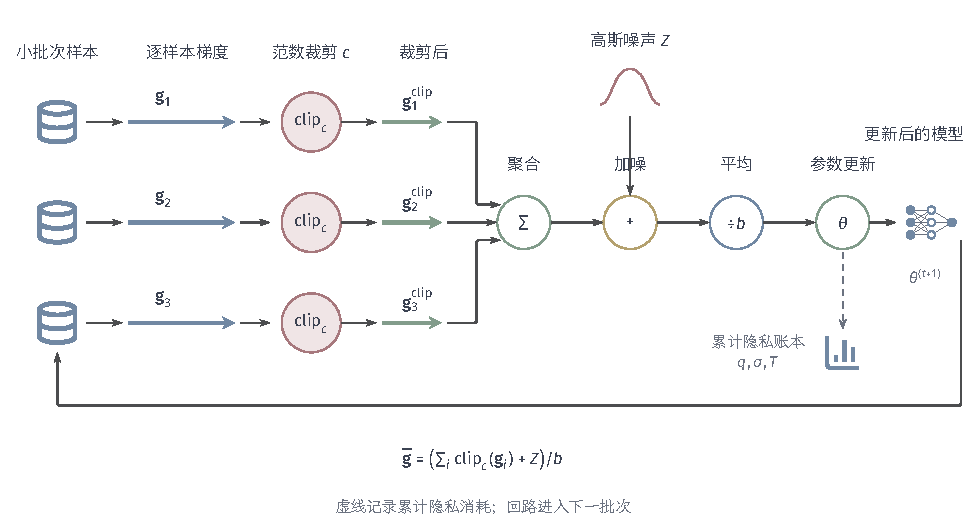
\includegraphics[width=164.600mm]{figures/03-foundations/03-trustworthiness/tikz/dp-sgd-update/figure.pdf}
  \caption{DP-SGD的一次更新。分别计算批次梯度$\bm g_i$，按$c$取$\operatorname{clip}_c(\bm g_i)=\bm g_i\min\{1,c/\lVert\bm g_i\rVert_2\}$，随后求和、加入高斯噪声$\bm Z$、除以$b$并更新。账本结合抽样率$q$、噪声尺度$\sigma$、步数$T$等累计消耗，分析必须对应保护单位、邻接关系和抽样约定。向量长度及高斯曲线只示意机制。}
  \label{fig:dp-sgd-update}
\end{figure*}

裁剪和加噪都有代价。裁剪使单样本影响有界，但也可能把有用的大梯度压小而引入偏差；加噪降低了更新的可区分性，同时干扰优化。用户级方案还要控制同一用户的总贡献，不能把他多条记录经逐记录裁剪后的贡献无限制相加。

噪声通常写为$\bm Z\sim\mathcal N(\bm0,\sigma^2c^2\bm I)$，其中$\sigma$称为噪声乘子，表示噪声标准差是裁剪阈值的多少倍。实现中批次往往不是固定的$b$条，而是对每条记录独立以概率$q$决定是否入选（泊松抽样），批量大小随之随机。这种抽样还有一个好处：一条记录在某一步很可能根本没被抽中，观察者面对的不确定性更大，因此每步的隐私消耗小于不抽样的情形，这称为抽样带来的隐私放大。泊松抽样的一种明确机制按数据集大小$n$和期望批量$qn$归一化；改成按实际批量归一化或固定大小不放回抽样时，要按实现重写机制、重新匹配邻接和抽样会计，不能直接套用固定$b$的公式。Abadi 等用矩会计（moments accountant）跟踪深度训练对数据的重复访问；实践中也常用第~\ref{sec:privacy-repeated-use}节的 Rényi 会计合并各步消耗。

比较优化效果和隐私参数时要分开看。固定抽样率$q$、噪声乘子$\sigma$、步数$T$和邻接约定，改变裁剪阈值$c$并让噪声按同比例缩放时，隐私界通常不变，因为它只取决于噪声尺度与敏感度之比$\sigma$；但优化轨迹会变：$c$过小会压掉更多梯度，$c$过大则增加绝对噪声量。批量变大也会同时改变平均更新的信噪比、抽样率和完成同样轮数所需的步数，必须固定训练预算口径才能判断隐私是否真的改善。

公开预训练有助于保留效用：只要预训练没有使用本次受保护的数据，隐私会计就从后续的私有数据访问开始；冻结部分参数能省计算，其余更新仍需裁剪和完整分析。如果模型选择、构造词表或筛选样本用了私有数据，这些前置步骤也属于发布算法的一部分，不能因为发生在梯度下降之前就不计入。

\paragraph{限制监督标签中的私人知识}

对大模型的每次更新都加噪，效用损失可能太大。另一种架构是不让私有数据直接参与发布模型的训练，而让持有私有数据的模型只回答有限的、受保护的监督查询。\term{教师集成的私有聚合}（PATE）把敏感数据切成互不重叠的分区，每个教师模型只用其中一片训练；学生模型用非敏感输入向教师们提问，从加噪后的投票结果中学习标签。被保护的接口是聚合后的投票，单个教师从不发布\scite{papernot2017pate}。

为什么投票容易分析？记第$j$类的教师票数为$v_j(\bm x)$，一种聚合方式是返回$\arg\max_j\{v_j(\bm x)+Z_j\}$，其中$Z_j$是加在各类票数上的独立噪声。在固定分区规则下，一条记录只出现在一个分区，至多影响一个教师的一票；这一票从一类改到另一类时，一类减一、另一类加一，票数向量的$\ell_1$变化至多为2，这就是聚合的敏感度。该界只依赖数据隔离，不要求教师模型具有凸性等性质。如果一个用户的数据跨多个分区，他就能改变多位教师，必须重新计算用户级影响。

隐私代价还与教师们的共识程度有关。共识很高时，一票改变不了答案，隐私代价小；近乎平票时，一票更容易翻转结果，代价大。可扩展 PATE 据此加入一个门控：先用带噪的共识阈值判断教师是否足够一致，只回答高共识的查询，再用投票差距细化隐私会计。“回答还是拒绝”本身也依赖私人数据，因此门控决定同样要计入隐私消耗\scite{papernot2018pate}。

拒绝低共识查询会改变学生能学到什么：罕见邮件可能更难达成教师共识，从而更常被拒答，因此要按群体检查获得标签的比例和学生效用。完整顺序是：先训练保持私有的教师，再对来源明确的非敏感输入查询带噪标签，最后训练学生，每一批新查询都计入访问。与 DP-SGD 比较，PATE 把保护接口放在监督标签上，教师内部算法可以不同，但需要适合学生的非敏感输入，并受查询数和共识不足的限制；DP-SGD 直接控制私有更新，不需要教师分片。比较两者前要先统一保护单位，最终噪声数值本身不能单独代表保护强弱。

学生训练完成后还需要加噪吗？如果学生只使用公开输入、受保护标签和独立随机性，那么给定这些标签后它与私人数据条件独立，可以直接套用第~\ref{sec:privacy-repeated-use}节的后处理性质，无需再加噪。但如果学生继续读取教师、原始记录或其他依赖私有数据的状态，就产生了新的、需要会计的访问。

图~\ref{fig:pate-private-teachers}示意教师与学生之间的边界：公开查询输入经加噪聚合得到受保护标签供学生学习，私有样本不直接交给学生。

\begin{figure*}[!htb]
  \centering
  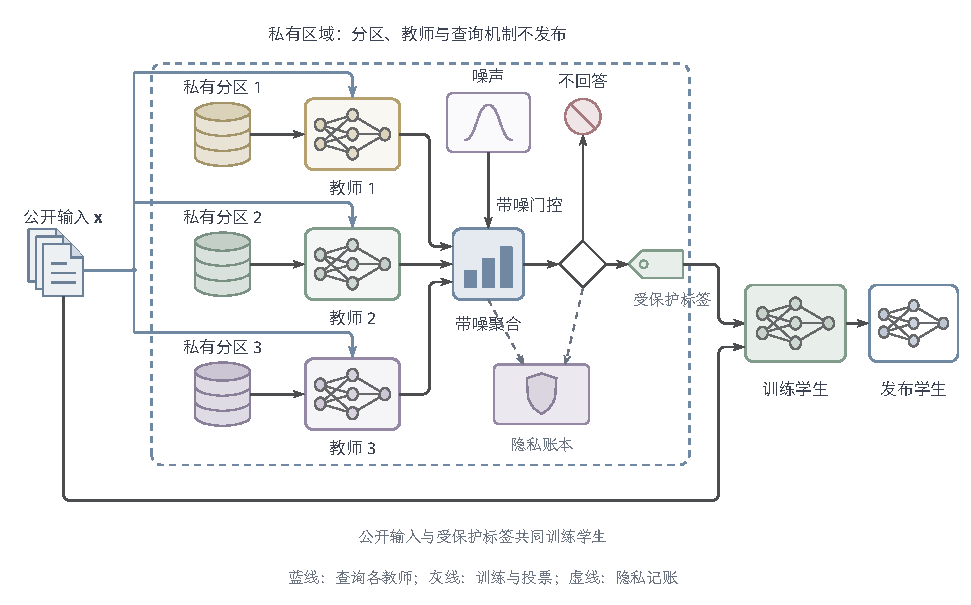
\includegraphics[width=164.600mm]{figures/03-foundations/03-trustworthiness/tikz/pate-private-teachers/figure.pdf}
  \caption{PATE的信息流。各教师用互不重叠的私有分区训练并保持不发布，非敏感公开输入取得各教师投票。加噪聚合和带噪门控产生受保护标签，低共识可不回答；两项决定均计入查询隐私消耗。学生仅以公开输入和受保护标签训练后发布，不能接触私有样本或单个教师。条形表示投票机制，不是实测数值。}
  \label{fig:pate-private-teachers}
\end{figure*}

\paragraph{协作方可见的中间更新}
\label{sec:privacy-collaborative-computation}

以上两种方法保护的是最终发布物。协作训练还有一种情况没有覆盖：服务器或其他客户端可能在模型发布前就看到各方的中间更新，第~\ref{sec:privacy-leakage-audit}节的梯度重构说明这些更新可能透露输入。因此要先列明各方权限和允许串通的范围，再决定如何隐藏中间信息。

几类密码学与硬件技术对应不同假设。安全聚合让服务器只能看到多个参与者更新的总和；安全多方计算（secure multi-party computation, MPC）和同态加密（homomorphic encryption, HE）让各方在只暴露受限中间信息的情况下完成指定计算；可信执行环境（trusted execution environment, TEE）依赖隔离执行的硬件假设。它们解决的都是“计算过程保密”；如果最终模型本身记住了私人内容，输出端的泄露仍要另行分析。

安全聚合的核心思想可以用两个客户端说明：两者事先共享一个随机向量$\bm r$，客户端一上传$\bm u_1+\bm r$，客户端二上传$\bm u_2-\bm r$。服务器单独看任何一条消息都只看到被随机掩码遮住的向量，相加时掩码抵消，得到$\bm u_1+\bm u_2$。Bonawitz 等把这一思想扩展到大量客户端，处理了部分客户端中途退出后掩码无法抵消的问题，并按对手能力和串通条件分析了“服务器能得到总和、却得不到任何单项更新”的范围\scite{bonawitz2017secureaggregation}。

即使只泄露总和也可能出问题。如果其他参与者的贡献已知、只剩一名未知者，观察者就能从总和确定这个人的贡献；对一群高度重合的人做多轮统计，也可能通过作差推断。因此参与人数、串通阈值和发布规则必须与安全聚合一起说明。分布式加噪还要证明噪声由谁产生、至少多少诚实参与者参与、有人退出后总噪声是否仍然足够。

第一部分的图~\ref{fig:federated-learning-process}区分了本地记录、上传更新和中心聚合：记录虽留在设备上，更新仍是由私人数据产生的可观测物，要按上述权限和串通条件检查。联邦学习把计算移到数据所在地，本身并不提供任何隐私保证。在联邦学习中，本地的记录级 DP-SGD 与“裁剪每个客户端的总更新”的用户级方案保护单位不同；信任中心时可以在安全聚合的总和上由服务器加噪，不信任中心时则需要客户端共同提供足够噪声或改用其他信任安排。

\subsection{结果发布与预测使用中的保护}
\label{sec:privacy-statistical-release}

开放模型权重、只开放受限查询、发布统计表，给接收者的观察能力差别很大。发布前应逐项确认实际可见内容：删掉无关分数、原始字段和调试信息可以收窄直接暴露；限制接口和查询数能减少某些攻击的观测。但这些操作本身不能推出差分隐私，要宣称差分隐私，仍须针对相应机制做分析。本小节先给出发布统计量的基本机制，再处理预测时的新输入，最后讨论多次发布怎样累计。

\paragraph{发布统计量中的个体影响}

即使可信管理者已经持有明文，仍要控制公开统计量对个人的暴露：小群体的精确统计，或对同一数据反复做差分查询，即使不含原文也能确定个人取值。第~\ref{sec:privacy-guarantees}节已经说明，解决办法是让发布值随机化。剩下的问题是噪声应该加多大：加少了保护不足，加多了统计量失去用处。

答案取决于一条记录最多能让统计量改变多少。设要发布实值统计$F(D)$，在给定相邻关系下定义其敏感度
\[
 \Delta F=\sup_{D\sim D'}\lvert F(D)-F(D')\rvert,
\]
即所有相邻数据对中统计量差值的最大者。计数的敏感度为1，因为增删一条记录最多让计数变化1。有了敏感度，就可以按比例选择噪声。拉普拉斯机制为
\begin{equation}
 M(D)=F(D)+Z,\qquad
 Z\sim\operatorname{Laplace}(0,\Delta F/\epsilon),
 \label{eq:privacy-laplace}
\end{equation}
其中尺度为$\beta$的拉普拉斯分布密度为$\frac{1}{2\beta}\exp(-\lvert z\rvert/\beta)$，是一个以0为中心、向两侧指数衰减的尖峰分布，这里$\beta=\Delta F/\epsilon$。机制要求$\epsilon>0$且$0<\Delta F<\infty$。两个边界情形需要单独处理：敏感度为零时统计量对相邻变化本来就不变，无需加噪；敏感度无界时必须先限定数据域或贡献，或换用其他机制，不能硬套一个有限的拉普拉斯尺度。

为什么这个噪声尺度恰好给出纯$\epsilon$-差分隐私？在同一输出值$u$处，$M(D)$和$M(D')$的密度分别为$\frac{1}{2\beta}\exp(-\lvert u-F(D)\rvert/\beta)$和$\frac{1}{2\beta}\exp(-\lvert u-F(D')\rvert/\beta)$，两者之比为
\[
 \exp\left(
 \frac{\lvert u-F(D')\rvert-\lvert u-F(D)\rvert}{\Delta F/\epsilon}
 \right)\leq e^\epsilon.
\]
不等号来自三角不等式：$\lvert u-F(D')\rvert-\lvert u-F(D)\rvert\leq\lvert F(D)-F(D')\rvert\leq\Delta F$，代入后指数不超过$\epsilon$。密度比处处不超过$e^\epsilon$，对任意输出事件积分，概率比也不超过$e^\epsilon$，即得到$\delta=0$的差分隐私不等式。这条推导说明噪声尺度必须从最大数据影响推出，不能先随便加噪再给它安一个隐私参数。

图~\ref{fig:trust-dp-neighbors}用相差一条记录的两个计数（3和4）比较随机发布：各自加同尺度的拉普拉斯噪声后，输出分布高度重叠，观察者拿到一次随机输出无法确定它来自哪个计数。两行是“二选一”的替代发布，不是同时发布两次。

\begin{figure*}[!htb]
  \centering
  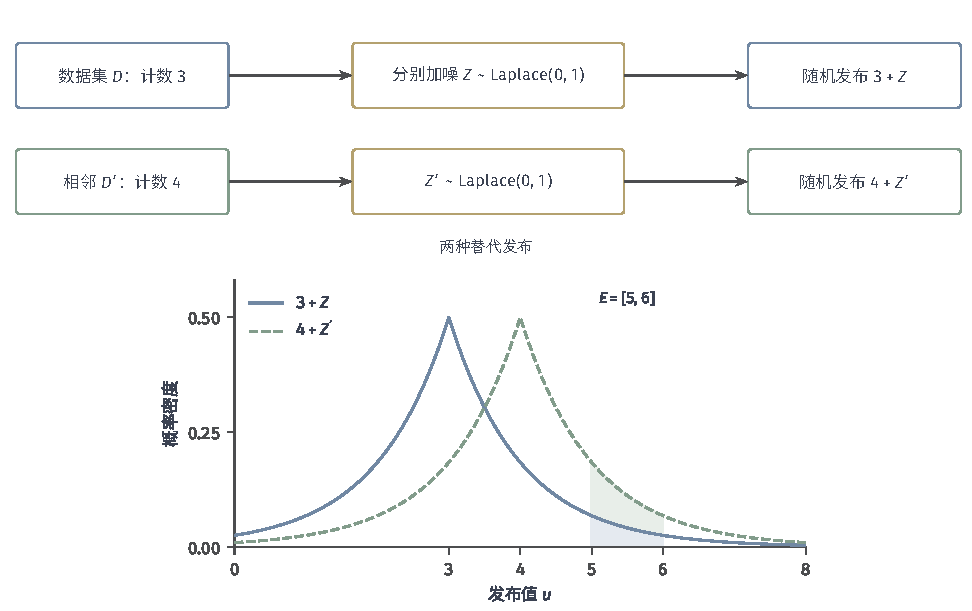
\includegraphics[width=164.600mm]{figures/03-foundations/03-trustworthiness/matplotlib/trust-dp-neighbors-comparison/figure.pdf}
  \caption{相邻计数的随机发布。两数据集仅差新增一条记录，准确计数为3和4；各反事实机制都使用尺度1的拉普拉斯分布，故$\Delta F=1$、$\epsilon=1$、$\delta=0$。两行是替代发布情形，不表示共同发布两次，也未规定联合耦合。每一行由准确计数经加噪得到随机发布，下方实线与虚线为解析密度，阴影比较同一事件$E=[5,6]$；横轴只画部分范围。一次输出的保护须对全部相邻数据和全部事件成立，曲线重叠只是示意。}
  \label{fig:trust-dp-neighbors}
\end{figure*}

把数字代入邮件例子。关键词邮件数每条记录贡献至多1，记录级敏感度为1；取$\epsilon=0.5$时加入尺度2的拉普拉斯噪声，相差1的两个计数产生大幅重叠的输出，不能再由一个准确整数判定目标邮件是否存在。若改为保护一名用户、每人最多贡献10封相关邮件，敏感度升到10，同样$\epsilon=0.5$要求噪声尺度20，除非另外限制每人贡献。保护单位变大，噪声和效用代价随之成比例增加。

\begin{example}[计数与平均值的不同要求]
\label{ex:privacy-sensitivity}
示例~\ref{ex:privacy-sensitivity}说明不同统计量的敏感度不能混用。在增加或删除一条记录的相邻关系下，人数计数的敏感度为1。均值需要另一组条件：固定$n$条记录、按“替换一条记录”定义相邻，且数值预先限定在$[0,1]$。此时替换一条记录使总和至多变化1，均值至多变化$1/n$。取消值域限制，一个极端值就能让均值改变任意多，敏感度无界。两例的邻接约定不同，不能因为“都是统计量”就用同一个噪声尺度。
\end{example}

\paragraph{预测上下文与结果接收者}
\label{sec:privacy-inference-context}

上面的机制保护的是训练数据或数据库。预测阶段还会产生新的信息流：检索私人文档、调用工具、保存对话日志，都会把敏感内容送入新接口。即使训练发布机制满足保护训练样本的差分隐私，模型收到一封新邮件后直接转给外部工具，仍会泄露这次请求。上下文进入模型、字段进入工具、结果交给接收者，各有各的信息边界，训练保证不会自动覆盖新增输入。

对应的措施是逐处收窄：检索前做权限控制，只把用户有权查看的文档送入上下文；工具只接收任务必要的字段；回复和工具请求要核查接收范围；日志限制保存内容。如果这些输入也承诺形式保护，新访问必须纳入所用机制的分析。输出过滤能拦下已知标识或固定模式，但会遗漏改写和间接推断，也可能误删合法内容，须分别用结果检验和过程核查确认。过滤器经测试有效，并不足以宣称上下文获得了形式化隐私保证。

\paragraph{多次发布的累计保护强度}
\label{sec:privacy-repeated-use}

一个系统很少只发布一次：统计表定期更新，训练有几千步，服务持续回答查询。观察者可以把多次结果联合起来推断，因此要回答两个问题：哪些后续操作不增加隐私消耗，哪些操作的消耗怎样累加。

先看不增加消耗的情形。已有发布$M(D)$之后，如果后续映射$K$只使用$M(D)$、公开信息和独立随机性，也就是给定$M(D)$后与原始数据$D$条件独立，那么$K(M(D))$满足与$M$相同的隐私参数。这称为后处理性质。理由是：观察者对$K(M(D))$做的任何检验，都可以改写成对$M(D)$的一个随机检验，而后者已受式~\eqref{eq:privacy-dp-definition}约束。例如把已经发布的计数拿去画图、换单位显示，不新增预算。但如果$K$另外读取了由$D$生成、却没纳入$M(D)$保证的缓存、模型或统计量，就引入了新的数据依赖，不能套用后处理性质。

如果每一步都重新读取数据运行机制，就需要组合（composition）分析。最基本的组合界把各步的$\epsilon$和$\delta$分别相加。例如同批邮件以$\epsilon=0.5$发布计数，若重新抽噪发布三次，基本组合给出纯差分隐私上界1.5。这些结果即使分散在不同网页或功能里，也不能拆开忽略，会计要覆盖观察者能联合看到的所有结果。自适应情况下，后一步的机制可以依赖前面的输出，此时要求每一步在给定此前所有输出后，仍对同一邻接关系满足所声称的条件界。只查询已发布的私有模型而不新增数据访问，与每次都重读私人上下文，是两种不同的过程。

训练更新往往有几千步，每步都先转成$(\epsilon,\delta)$再直接相加，得到的界过于宽松，需要更紧的会计工具。思路是换一种度量两个输出分布差异的方式，使它在组合时相加且不损失精度。记要比较的两个输出分布为$P,Q$，阶数$\alpha>1$，当$P$关于$Q$绝对连续（记$P\ll Q$，即$Q$下概率为零的事件在$P$下也为零）时，Rényi 散度定义为
\[
 D_\alpha(P\|Q)=\frac{1}{\alpha-1}\log\mathbb E_{Q}\left[\left(\frac{\mathrm dP}{\mathrm dQ}\right)^{\alpha}\right],
\]
它用密度比$\mathrm dP/\mathrm dQ$在$Q$下的$\alpha$阶矩衡量两个分布差多远；两个分布相同时为0，绝对连续性不成立或该阶矩无穷时取$+\infty$（背景可参考\BookChapterRef{chap:information-theory-and-statistical-geometry}{卷2《数学准备：概率、因果与决策》的“概率分布的分析与优化”章}）。

\term{Rényi差分隐私}（Rényi differential privacy, RDP）要求：在声明的邻接关系下，对每一对相邻数据集，输出分布的某阶 Rényi 散度都不超过同一个上界。用$P_D$表示$M(D)$的输出分布，就是对所有相邻的$D,D'$满足$D_\alpha(P_D\|P_{D'})\leq\rho(\alpha)$。这里固定了保护单位、阶数和统一上界，不能只挑平均的几对数据检查\scite{mironov2017rdp}。

RDP 的好处在于组合规则简单：如果第$t$步在同一邻接关系下、给定任意此前输出后都有统一的$\rho_t(\alpha)$界，那么完整输出序列的 RDP 上界就是各步之和$\sum_t\rho_t(\alpha)$。最终报告通常仍需$(\epsilon,\delta)$形式，事先选定$\delta\in(0,1)$后可以转回：
\begin{equation}
 \epsilon(\delta)=
 \inf_{\alpha>1}\left\{
 \sum_{t=1}^{T}\rho_t(\alpha)
 +\frac{\log(1/\delta)}{\alpha-1}
 \right\}.
 \label{eq:privacy-accounting}
\end{equation}
花括号里第一项是累计的散度，随$\alpha$增大而增大；第二项是换算成$(\epsilon,\delta)$时付出的代价，随$\alpha$增大而减小。取下确界就是在两者之间找最合适的阶数。这个选择只在已经证明有效的阶数界中进行，不读取私有数据，因此不产生额外消耗。

以不含抽样的高斯机制为例，有$\rho(\alpha)=\alpha\Delta_2^2/(2s^2)$，其中$\Delta_2$是向量统计的二范数敏感度，$s$是逐坐标噪声标准差。$T$步相同的高斯更新累计为$T\alpha\Delta_2^2/(2s^2)$，代入式~\eqref{eq:privacy-accounting}后，$\epsilon$大致随$\sqrt{T}$而不是随$T$增长，这正是它比逐步相加更紧的原因。加入抽样会改变整条$\rho(\alpha)$曲线，不能简单把抽样率乘到最终$\epsilon$上；独立泊松抽样和固定大小不放回抽样需要不同的放大分析；如果选哪些样本本身依赖私有数据，也不能沿用数据独立抽样的放大结论。

\section{数据撤回与模型消除}
\label{sec:privacy-unlearning}

前面各节假设数据一直留在系统中。用户撤回邮件后，系统面对的是另一个问题：怎样把这些指定记录对模型的训练影响移除。这称为\term{机器遗忘}（machine unlearning）。本节的“模型消除”特指这一目标，不是删除或停用整个模型。这里要分开三件事：清除原始文件、阻止模型再输出某内容、消除记录对训练的影响，三者各有各的验收对象。

\paragraph{遗忘的参照标准}

“影响已经移除”需要一个可比较的参照。用$A$表示训练映射，$D$是原训练集，$F$是待撤回记录集合，$U$是模型更新程序。图~\ref{fig:trust-privacy-deletion}区分了“删数据”和“更新模型”：从数据集中删除记录得到$D\setminus F$，并不会改变已经训练好的模型$A(D)$；更新程序$U$的产出，应与“从未用过$F$、从头训练得到的模型$A(D\setminus F)$”比较（为简洁省略随机参数）。一个提取测试没恢复出私人片段，只支持该测试本身，不能说明全部训练影响都消失了。

\begin{figure*}[!htb]
  \centering
  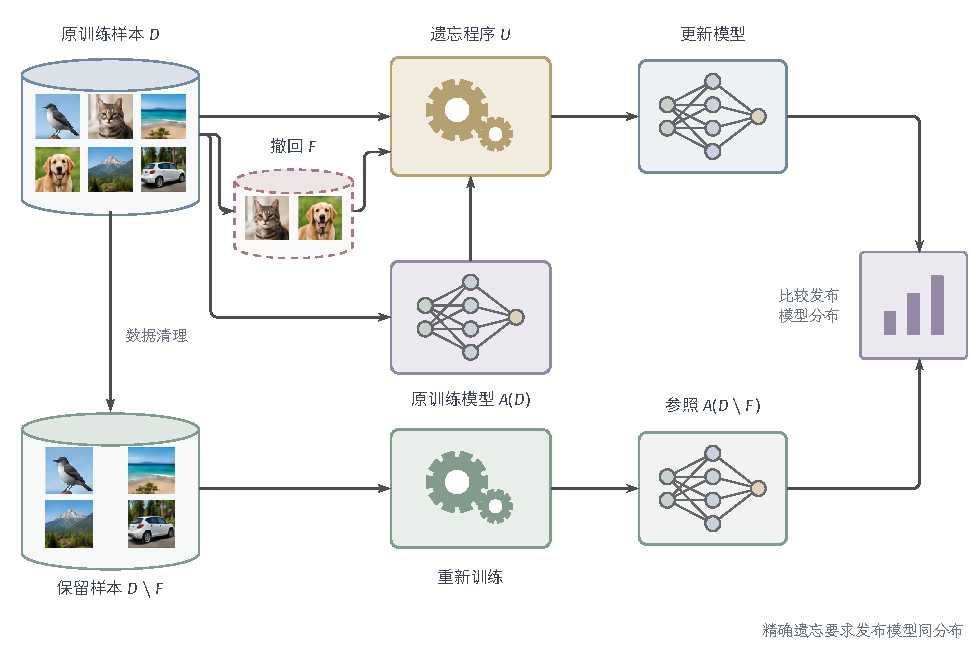
\includegraphics[width=164.600mm]{figures/03-foundations/03-trustworthiness/tikz/unlearning-reference/figure.pdf}
  \caption{数据清理与训练影响消除。删除记录得到$D\setminus F$，原训练模型$A(D)$仍保持原状态；$U$另外读取原训练模型、原训练样本和撤回集合进行更新。应比较更新结果与从未使用$F$的重训练模型分布：精确遗忘要求同分布，近似遗忘需指定距离或可区分性标准。}
  \label{fig:trust-privacy-deletion}
\end{figure*}

先在一个明确的观察视图下给出标准：集合差按记录身份定义，并限定观察者只拿到替换后的新发布模型，不再持有旧模型、旧回复、日志或其他辅助状态。在这个视图内，精确遗忘要求
\begin{equation}
 U(A(D),D,F)\ \overset{\mathrm d}{=}\ A(D\setminus F).
 \label{eq:privacy-exact-unlearning}
\end{equation}
$\overset{\mathrm d}{=}$表示同分布：训练和遗忘过程都有随机性（初始化、数据顺序等），左右两边各自是一个“已发布模型”的分布，要求两者相同；它不是要求某个固定模型对单个请求的预测分布相同\scite{bourtoule2021sisa,guo2020certifiedremoval}。如果观察者还能同时拿到旧模型、旧回答或其他状态，就要比较整个联合观察分布：让新模型的分布与参照相同，并不能收回已经披露出去的信息。程序可以保存额外的内部状态，但这些状态若可见，也必须纳入参照。

精确同分布往往代价太高。近似遗忘把它放宽为“在指定距离或可区分性标准下足够接近”。也可以改成比较参数、预测或特定攻击的结果，但这些只考察模型经过某个观察映射后的量；只在少量请求上结果接近，除非另有证明，不能推出整个发布模型分布都接近重训练结果。

遗忘和差分隐私比较的对象不同。差分隐私训练限制“一条记录参与与否对输出的影响”，是事前对所有记录的统一约束；遗忘比较的是“撤回后更新的模型”与“从未用它训练的模型”，是事后针对指定记录的处置。两者可以配合，差分隐私训练常常让遗忘更容易，但使用了差分隐私不能单独证明某次具体撤回已经完成。

一次撤回的完整流程是：先确定范围、停用相关数据、清理可控制的副本和衍生状态、隔离暂时无法清除的部分；数据若已进入训练结果，再在完整重训练、局部重算和参数修正中选一个满足遗忘标准的方案（三者互为备选）；正式处置完成前用输出限制作过渡；最后分别验收数据资产、接口和模型影响，并记录整个流程的时间与资源。以下四小节依次展开。

\subsection{撤回范围与数据资产清理}
\label{sec:privacy-asset-deletion}

定位撤回范围时，利用稳定的记录标识、用户关联和计算依赖，找出原始文件、清洗副本、特征缓存、检索索引、向量记录、训练快照和相关日志。用户级撤回不能只删账户表里的一行；一条记录涉及多人时，还要说明删除整条还是只删某些字段。范围确定后，后续处置才有可核对的清单。

快速响应依赖事先保存的数据去向记录：记录与数据版本、索引项、训练任务、模型版本之间的映射，可以用来生成撤回任务。确认请求后，先阻止数据再进入训练队列、从在线检索范围移除索引项、禁止产生新副本；再按存储依赖清单删除或重建，并核查正在运行的任务有没有使用旧快照。删除标记可以停止正常使用，物理副本真正清除是另一个完成状态。

清理顺序要与模型更新协调，因为某些遗忘算法还需要读撤回记录：扣除贡献需要它的统计量，参数修正需要它的损失。若必须读原文，可在受限的撤回环境中完成后再删除工作副本；已有统计状态够用时可以免读，但这些状态本身也要核查是否含私人信息。停止用于训练和检索，不等于立刻销毁算法还需要的输入；临时副本的权限、存续期和最终清除都属于本次验收。

删除索引还要处理衍生缓存：文档移除后，它的向量、片段缓存和生成的摘要可能仍被检索或复用；从备份恢复时，要依据已保存的撤回记录重放相应删除，防止旧数据回流。无法立即逐条清理的归档，要明确隔离、清除计划和恢复限制。“在线接口查不到了”只描述当前接口状态，不能表述为所有副本都已消失。

按存储和依赖清单验收时，逐项区分已完成、待处理和无法控制的副本，测试记录是否还能被检索、导出或进入训练，并绑定模型版本。审计日志要能证明处置过程，但应避免再次保存完整私人内容。资产清理解决的是“仍被保存和再使用”的问题，参数中残留的训练影响留给下一小节。

\subsection{训练影响的消除方案}
\label{sec:privacy-unlearning-methods}

已经参与训练的记录，要按遗忘标准、算法结构和可用状态选择消除方案。完整重训练直接生成参照；局部重算利用可追踪的计算结构，只重做受影响的部分；参数修正从旧模型出发，近似求删除后的结果。三者条件和证据不同，“耗时少”只说明计算节省，不能单独代表遗忘充分。

\paragraph{完整重训练}

完整重训练在$D\setminus F$上重新运行$A$，直接产生式~\eqref{eq:privacy-exact-unlearning}右侧的参照分布，代价是要再处理一遍全部保留数据。它比较的是同一流程下的模型分布，不要求某一组随机参数恰好重现旧结果。

“重新运行$A$”的范围比训练循环更大：词表、标准化、样本筛选和模型选择若依赖撤回记录，就要在排除$F$后重算；受$F$影响的优化器状态或初始化检查点不能当作“从未读过$F$”的起点。公开预训练或中间结果只有确定独立于$F$时才能复用；早停轮数、随机抽样等训练规则都属于$A$，要一起固定。

新模型完成后还要切换服务、使旧缓存失效，并记录它覆盖了哪些撤回请求。多个撤回请求可以合并以省去重复训练，但等待期间仍要限制旧数据和旧服务的暴露，并报告实际等待时长。“进入批处理队列”只是安排，不能据此把模型影响标为已消除。

\paragraph{局部重算}

重训练的代价促使我们问：一条记录到底影响了哪些计算？模型若只依赖少量可更新的统计量，可以直接扣除该记录的贡献；训练若事先被隔离成多个部分，可以只重算受影响的部分。两种节省都依赖已知的计算结构，不意味着能在任意神经网络参数中定位某条记录。

Cao 和 Yang 把学习过程组织成可更新的求和形式，撤回时修改对应统计量即可，减少对保留数据的重复处理\scite{cao2015unlearning}。最简单的例子是只用记录数$n$和数值和$S$计算均值$\hat\mu=S/n$。撤回$m<n$条、其和为$S_F$后，可以直接更新为
\[
 \hat\mu_- =\frac{S-S_F}{n-m}.
\]
它在数学上完全等于对保留数据重新求均值（实现上仍有浮点误差）。例如从$\{1,2,3\}$删除3，更新为$(6-3)/(3-1)=1.5$。这说明特定统计模型可以精确扣除贡献，但不能推广成“深度训练中把某个梯度减回去就行”：深度训练的每一步都依赖先前的参数，撤回记录的影响会沿优化轨迹传播到后续所有步。采用贡献扣除的前提是算法和前置处理确实符合求和结构，且能追踪衍生数据依赖。

另一种思路是在训练前就隔离依赖。SISA（sharded, isolated, sliced, and aggregated training，即分片、隔离、切片、聚合）把数据分成若干片，每片独立训练一个子模型；片内再把数据按顺序分成切片逐个训练，并在每个切片结束时保存检查点；预测时聚合各子模型的输出。删除记录时，只需回到它首次进入之前的检查点，再重算后续切片\scite{bourtoule2021sisa}。

例如邮件预先分四片，每片含三个顺序切片，待删记录在第二片的第二切片。其他三个子模型原样保留，第二片从第一切片末的检查点出发，在排除该记录后重算后两个切片。节省来自依赖隔离，而不是从最终参数里把记录影响“抽出来”。如果标准化、词表和模型选择仍在全数据上共同计算，就构成跨片依赖，必须一起处理。

分片也有代价。分片增多会减少每个子模型的数据，可能降低集成相对整批训练的效用；检查点越密，存储和敏感状态管理成本越高。因此评估不能只看单次删除耗时，还要计入初训、状态保存、常见请求分布和保留任务效用，并检验最坏的请求位置，即在给定删除条数下使受影响分片数或重算时间最大的情形。SISA 更新的参照也必须采用同样的分片、切片和聚合规则，并核对删除后抽样和随机状态的处理；整批训练的单一模型本来是另一种训练算法，不能用与它的比较宣称 SISA 的输出分布与之相同。

\paragraph{参数修正与近似遗忘}

如果依赖没有事先隔离，就只能从当前参数出发，近似求删除后应有的模型。这时要警惕一个误读：参数改变量小，不能直接说明指定记录的影响已被充分消除，必须另有误差和分布依据。

Guo 等的认证删除为一类正则化线性模型给出可证明的近似误差控制：用一步牛顿更新逼近删除后的解，再靠训练目标中预先加入的随机扰动遮掩剩余误差\scite{guo2020certifiedremoval}。保证依赖强凸性、光滑性等条件，只有“删除后梯度残差很小”还不足以证明删除成功。

先看牛顿更新在优化上做什么。原参数$\hat{\bm\theta}$是全数据目标的最优点；删除记录后目标变成$L_-(\bm\theta)$，设它光滑且强凸，$\hat{\bm\theta}$不再是它的最优点。在$\hat{\bm\theta}$处把$L_-$做二次近似，其梯度和海森矩阵分别为$\bm g_-$和$\bm H_-$，令二次近似的梯度为零，得到一步牛顿更新
\begin{equation}
 \tilde{\bm\theta}
 =\hat{\bm\theta}-\bm H_-^{-1}\bm g_-.
 \label{eq:privacy-newton-removal}
\end{equation}
当目标在解附近接近二次函数时，这一步能消除主要偏差。剩余误差有多大？设$L_-$在无约束可微条件下是$\lambda$-强凸的（$\lambda>0$），删除后最优解为$\bm\theta_-^*$。强凸性意味着任意两点梯度之差至少是距离的$\lambda$倍，而最优点处梯度为零，于是
\[
 \lambda\lVert\tilde{\bm\theta}-\bm\theta_-^*\rVert_2
 \leq\lVert\nabla L_-(\tilde{\bm\theta})-\nabla L_-(\bm\theta_-^*)\rVert_2
 =\lVert\nabla L_-(\tilde{\bm\theta})\rVert_2 .
\]
即参数误差不超过更新点梯度范数除以$\lambda$。但这个界控制的只是参数误差：确定性误差再小，观察者仍可能利用参数间的精细差别识别记录。因此认证还要把残差与训练时的随机扰动分布联系起来，证明输出按既定可区分性标准接近重训练。连续撤回要累计残差和认证预算，超出条件时靠重训练恢复承诺。非凸的大语言模型不具备上述强凸前提，不能直接套用这套线性分析。

没有认证条件时，深度模型只能做经验修正：在撤回样本上提高预测损失，以压低相应答案的概率；同时在保留数据上降低任务损失或约束预测变化。前者减少目标行为，后者限制附带损伤。如果只提高撤回样本的损失，模型也可能靠破坏一大片能力来达标，所以“撤回样本上准确率下降”不是衡量遗忘充分程度的单一指标。负偏好优化（negative preference optimization, NPO）针对这类更新的不稳定：以原模型为参考，按目标序列在当前模型和参考模型中的相对概率调节更新，目标序列已被明显压低时其权重自动下降，再结合保留数据损失限制效用下降\scite{zhang2024npo}。它给出的是经验修正路径，不保证更新后的参数分布接近完整重训。

第~\ref{sec:interpretability-local-training}节的局部影响近似可以用来估计修正方向，但大规模删除通常超出线性近似范围。数据归因解释的是样本如何影响行为，遗忘要求的是改后模型满足重训练参照标准；方向估计正确不足以提供后者需要的误差和分布界，多次删除还要核查近似误差的累积。

选择方案时先固定遗忘标准，再比较满足该标准的响应代价：完整重训练适用面广但成本高；统计贡献扣除和隔离训练利用结构节省重算；参数修正需要认证前提，否则只能给出经验边界。近似结果达不到标准时，应重训练或收紧服务范围。

\subsection{撤回完成前的过渡保护}
\label{sec:privacy-unlearning-output-control}

重训练或修正需要时间。在清理和模型更新完成前，可以先限制可控接口的暴露作为过渡：撤下检索文档、使缓存失效、减少敏感请求字段、拒绝无权接收者、屏蔽回复中的已知私人标识。这些措施能立即减少服务返回的内容。

但过渡措施不等于影响已经消除。在最终文本中过滤编号没有改变参数，改写编号、关联提问、其他接口或旧权重仍可能绕开；为拒答而微调虽然改了参数，也可能只是让模型避开某类问题，拒答增多不能单独证明训练影响消失；知识编辑改掉一个答案后，同样需要额外证据才能宣称指定数据的影响已接近重训练参照。

数据去向决定需不需要做训练影响消除。内容只存在外部检索库时，清除记录、索引和缓存就能切断来源；模型若也曾用这些内容训练，切断检索后参数里的问题仍然存在。检索源删除和输出过滤因此要分别验收，不能对所有请求套用同一种操作。

可以先执行输出限制、随后完成影响消除，两者的状态、接口和验收结果分别报告。本地更新不会自动删除已经交给外部的内容或别人持有的模型副本，因此承诺范围只能包括明确可控制的状态和服务。

\subsection{撤回结果与效率的验收}
\label{sec:privacy-unlearning-validation}

撤回验收分三项：清单内副本已删除或隔离、指定接口的临时限制已生效、模型影响已达到选定标准。若记录从未进入训练，第三项可记为“不适用”，但要留下数据流和版本证据。任一处遗漏都算撤回未完成：文件已删却仍在用受影响的旧模型，或模型已更新却又把旧样本送入下一轮训练。

模型项必须回到式~\eqref{eq:privacy-exact-unlearning}的参照，不能用“重算量小”或“参数改动小”判断。受控比较要固定撤回集$F$、剩余数据和训练规则，保留原模型、遗忘模型和用$D\setminus F$重训的模型，同时核查待消除信息和保留任务效用。

式~\eqref{eq:privacy-exact-unlearning}比较的是模型分布，要做经验比较，就必须独立重复训练和遗忘多次，报告重复实例数和估计误差。有限样本只支持选定统计量或可区分性的估计，精确同分布仍需形式证明。固定一个模型反复生成，只估计了该模型在给定请求和解码规则下的行为分布，并不是新的训练实例。两类分布证据都缺时，只能报告行为层面的结论。

行为评价要预先设定：同一设置内三种模型用相同的请求、解码和攻击预算；再跨设置改变提示、采样和预算做压力测试，分别报告。对项目编号邮件，可以比较提取成功率和成员分数，在保留邮件上测分类风险、概率校准和群体表现。随机生成在设置内用独立种子重复，给出次数和估计误差，避免把一次随机输出或表面拒答当成完整证据。

解释遗忘审计结果时要避免两个方向的错误。遗忘模型不再一字不差地复现项目名，只说明通过了精确匹配检查；改写提示、问关联事实、多轮问答仍可能暴露同一信息。反过来，用不含该邮件的数据重训的模型也可能从其他保留邮件里学到同一项目名。如果要求遗忘模型完全不能回答这条知识，就比“移除指定记录影响”更强，需要重新定义参照数据和知识范围，否则会把重训练模型本来就能知道的事实误判成遗忘失败。

成员推断用于遗忘审计时，参照也要调整。常规成员推断比较训练成员和从未参与的非成员；撤回记录曾经是成员，遗忘后它应接近“从未纳入该记录”的重训练参照，不能原样套用二类标签和阈值。如果遗忘过度、让撤回记录的损失异常高，反而会暴露“它曾被撤回”。正确做法是在遗忘模型和重训模型上比较同一撤回记录的分数分布，并检查相似的保留样本；“比其他所有样本都难预测”不能替代“接近重训练分布”的证据。

保留效用包括总体性能和语义相关的能力：删除某人的私人经历，不应无依据地让模型无法回答整个职业类别的问题；破坏校准还会影响第~\ref{chap:trust-reliability}章的决策风险。相同删除范围下应并列报告残留信息、保留风险、更新时间和状态存储，并区分理论保证与经验结果。

效率也要完整计量，它包含多个时延：从接受请求到停止使用、从停止使用到清完副本、从请求到新模型上线。参数修正的几秒钟没有计入定位、排队、重建索引、核验和版本切换。方法比较还要计入初训和额外存储，并固定删除规模、硬件和效用要求。连续撤回会累积近似误差；新旧版本联合可见时，新模型的单项保证收不回外部已经从旧模型获得的信息。完成记录因此要分别标识资产、过渡保护和模型影响三项。

\section{本章小结}
\label{sec:privacy-summary}

回到章首那封邮件。它可能暴露的不只是原文：成员身份、邮件内容和预测时新增的上下文是三种不同的秘密，可以分别经由原文存取、训练更新、发布参数和服务输出流出。隐私承诺因此先要写清涉及谁、哪些信息、允许谁接收。访问规则管住明文，差分隐私进一步限制一条受保护数据对发布结果分布的影响；它的强度由相邻关系所定的保护单位决定，记录级参数不能直接当作用户级保证，也不消除公开规律带来的推断。

检查承诺有两类证据。结果审计按属性推断、成员推断、内容提取和输入重构分别匹配攻击者知识和判据，攻击成功给出泄露证据并可推出参数下界，失败只说明在指定资源下尚未发现；过程核查沿数据流检验敏感度、噪声、抽样和会计等机制前提。形式保证需要定义、数学分析和实现三者同时成立。实现上，采集阶段减少无关输入并可在本地随机化，训练阶段用逐样本裁剪加噪或受保护的教师投票限制贡献，发布阶段按敏感度校准噪声并累计多次发布的消耗；协作计算的过程保密与输出保护要分别论证。

公平审计与隐私的张力可以在职责隔离、最小访问和受控发布下同时处理：公平验收保留充分的群体证据，隐私验收限制属性流向和统计发布，两项结果要同时报告。

撤回邮件时，先定位范围、清理数据资产；已参与训练的，再在完整重训练、局部重算和参数修正中选择，使模型满足以重训练为参照的遗忘标准。处置前的输出限制只能减少过渡暴露。最终分别核验资产、接口和模型影响，并报告保留效用和从请求到完成的响应时间。

本章假设观察者只是利用系统给出的信息。下一章把主动攻击者纳入分析，考察他们如何选择输入、污染训练或操纵工具来利用系统的薄弱位置；本章建立的信息边界、泄露证据和撤回参照，也将用于判断私人信息损害和恢复措施。

\paragraph{扩展阅读}

Dwork与Roth可补足差分隐私的机制、组合和统计代价，Abadi等则展示裁剪、加噪及重复访问会计怎样进入深度训练。对照阅读时应核对相邻关系与保护单位，尤其不能把记录级参数直接当成用户级保证\scite{dwork2014privacy,abadi2016dp}。

发布后的泄露与撤回可对照Carlini等的训练数据提取和Bourtoule等的SISA。前者研究查询怎样恢复训练片段，后者利用预定隔离减少删除重算。攻击失败的经验观察与接近重训练的分布要求，仍是不同证据\scite{carlini2021extraction,bourtoule2021sisa}。
